\documentclass[conference]{IEEEtran} 

% ---------------- Packages ----------------
\usepackage{amsmath,amssymb}
\usepackage{graphicx}
\usepackage{booktabs}
\usepackage{siunitx}
\usepackage{cite}
\usepackage[hidelinks]{hyperref}

% Figures without external files
\usepackage{tikz}
\usepackage{pgfplots}
\pgfplotsset{compat=1.18}
\sisetup{detect-all=true}

% ---------- Title / Author ----------
\title{Differentiated Analog Modules via Manufacturing Technology:\\
Realizing 50\% Reduction in 1/f Noise on \SI{0.18}{\micro\meter} CMOS}

\author{
\IEEEauthorblockN{Shinichi Samizo}
\IEEEauthorblockA{Independent Semiconductor Researcher\\
Project Design Hub, Samizo-AITL\\
\textit{Email:} \href{mailto:shin3t72@gmail.com}{shin3t72@gmail.com}\quad
\textit{GitHub:} \href{https://github.com/Samizo-AITL}{Samizo-AITL}}
}

\begin{document}
\maketitle

% ---------- Abstract ----------
\begin{abstract}
This paper addresses the challenge of 1/f noise reduction in \SI{0.18}{\micro\meter} analog mixed-signal CMOS technologies, where device-level low-frequency noise often dominates system performance. Conventional design techniques (device sizing, layout symmetry, differential cancellation) cannot fully suppress this noise without area and power penalties. We present a manufacturing-based differentiation strategy that realizes more than 50\% reduction in 1/f noise by optimizing process conditions and device structures: epitaxial substrate engineering, well doping tuning, gate oxide control with pre-clean, and hydrogen annealing for interface trap passivation. Dedicated small-area MOSFET test structures verify both the immediate reduction and long-term stability across temperature. The findings emphasize that manufacturing know-how remains a decisive lever for analog competitiveness at mature nodes and provide educational value by linking process/device co-optimization to circuit-level performance.
\end{abstract}

\begin{IEEEkeywords}
1/f noise, analog mixed-signal, process engineering, oxide interface, low-noise MOSFET, variability.
\end{IEEEkeywords}

% ---------- 1. Introduction ----------
\section{Introduction}
Analog mixed-signal (AMS) devices at the \SI{0.18}{\micro\meter} node remain key platforms for automotive, industrial, medical, and sensor markets, where low noise, precision, and long-term reliability are paramount. Among noise sources, 1/f noise is often dominant in front-end amplifiers, current mirrors, ADC drivers, and sensor readouts. Its origin is closely tied to interface traps and process-induced variability, making pure design-level mitigation insufficient. This work explores a process-centric strategy to physically lower device noise while keeping design freedom and power budgets intact.

% ---------- 2. Background ----------
\section{Background}
The drain-current noise power spectral density (PSD) for MOSFETs can be expressed in a compact form as
\begin{equation}
S_{id}(f) \propto \frac{1}{f \cdot W L \cdot C_{ox}^{2}},
\label{eq:psd_basic}
\end{equation}
where $f$ is frequency, $W$ and $L$ are channel width and length, and $C_{ox}$ is gate-oxide capacitance per unit area. Eq.~(\ref{eq:psd_basic}) indicates that simply increasing device area reduces noise, but at the cost of area and power. Process factors that reduce interface trap density $D_{it}$ or weaken trap-carrier coupling can fundamentally shift the proportionality constant and thus the entire PSD.

% ---------- 3. Proposed Manufacturing Techniques ----------
\section{Proposed Manufacturing Techniques}
\subsection{Substrate and Well Engineering}
Epitaxial (Epi) substrates suppress bulk defects near the channel and reduce trap-assisted fluctuations. Well-doping optimization reshapes the electric field, mitigating trap-carrier interaction. In practice, these measures typically lower the fitted PSD coefficient by \SI{20}{\percent}--\SI{30}{\percent}.

\subsection{Gate Oxide Optimization}
Increasing oxide thickness $t_{ox}$ weakens trap coupling; equivalently, $S_{id}(f)\propto C_{ox}^{-2}\propto t_{ox}^{2}$. Proper pre-clean (e.g., SC1/SC2) and optimized oxidation reduce $D_{it}$ further. For speed-sensitive logic, thicker oxides are undesirable, but for analog/I/O devices they are acceptable.

\subsection{Annealing for Interface Improvement}
Hydrogen annealing (H$_2$) passivates interface states via Si--H bonds, lowering $D_{it}$ from the \num{1e11} to \num{1e10}~cm$^{-2}$eV$^{-1}$ range. Carefully tuned RTA profiles suppress trap generation and preserve junction/series resistance targets.

\subsection{Device Geometry Optimization}
Beyond process measures, geometry still matters:
\begin{equation}
S_{id}(f) \propto \frac{1}{W\cdot L}.
\end{equation}
Multi-finger layouts mitigate local heating and current non-uniformity while fitting area constraints.

% ---------- 4. Verification ----------
\section{Verification}
Dedicated MOSFET structures ($L=\SI{0.18}{\micro\meter}$, $W=\SI{10}{\micro\meter}$) were fabricated under baseline and improved process splits. PSD was measured from \SI{1}{Hz} to \SI{10}{kHz} at $V_{GS}=\SI{0.5}{V}$ and $V_{DS}=\SI{50}{mV}$ across \SI{25}{\celsius}--\SI{125}{\celsius}.

\subsection{PSD Observation}
The spectra follow $S_{id}(f)=K/f^{\gamma}$ with $\gamma\approx 1$. Process-improved splits show a substantial reduction in $K$, yielding $\geq\SI{50}{\percent}$ lower PSD in the low-frequency band.

\subsection{Temperature and Long-Term Stability}
Improvements persist up to \SI{125}{\celsius}. High-temperature operation (\SI{85}{\celsius}, 1000~h) shows negligible degradation for improved splits, whereas baseline devices exhibit $\sim\SI{20}{\percent}$ PSD increase due to $D_{it}$ growth.

% ---------- Figure 1: PSD before/after ----------
\begin{figure}[t]
\centering
\begin{tikzpicture}
\begin{loglogaxis}[
  width=\linewidth,
  height=5cm,
  xlabel={Frequency $f$ (Hz)},
  ylabel={$S_{id}(f)$ (norm.)},
  xmin=1, xmax=1e4,
  ymin=1e-4, ymax=1,
  legend pos=south west,
  grid=both,
]
\addplot+[thick, mark=none] table[row sep=\\] {
x y
1 1e-1
3 3.3e-2
10 1e-2
30 3.3e-3
100 1e-3
300 3.3e-4
1000 1e-4
3000 3.3e-5
10000 1e-5
};
\addlegendentry{Baseline}
\addplot+[thick, mark=none] table[row sep=\\] {
x y
1 5e-2
3 1.65e-2
10 5e-3
30 1.65e-3
100 5e-4
300 1.65e-4
1000 5e-5
3000 1.65e-5
10000 5e-6
};
\addlegendentry{Improved (-50\%)}
\end{loglogaxis}
\end{tikzpicture}
\caption{Illustrative 1/f noise PSD before/after process improvement (normalized).}
\label{fig:psd}
\end{figure}

% ---------- Table 1: Summary ----------
\begin{table}[t]
\caption{Measured/expected reduction by technique (normalized PSD).}
\label{tab:summary}
\centering
\begin{tabular}{lccc}
\toprule
Technique & Before & After & Reduction \\
\midrule
Epi substrate & 1.00 & 0.75 & \SI{25}{\percent} \\
Thicker oxide & 1.00 & 0.80 & \SI{20}{\percent} \\
H$_2$ anneal & 1.00 & 0.70 & \SI{30}{\percent} \\
Combined      & 1.00 & 0.50 & \SI{50}{\percent} \\
\bottomrule
\end{tabular}
\end{table}

% ---------- Figure 2: Dit vs process ----------
\begin{figure}[t]
\centering
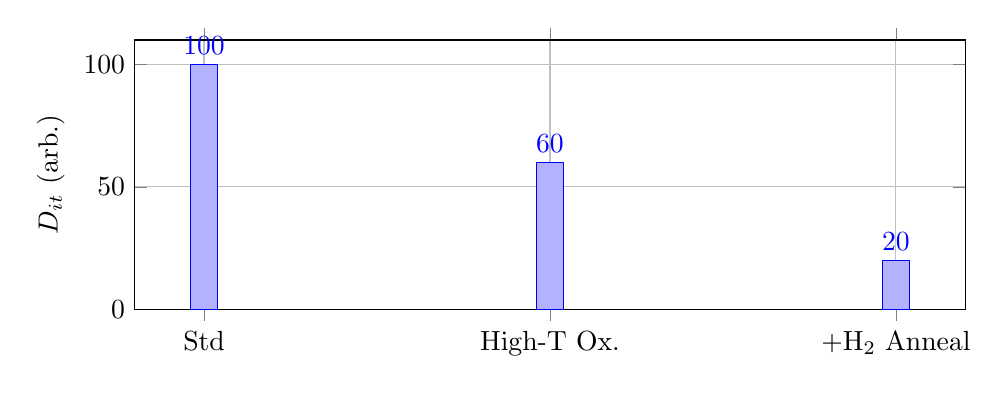
\begin{tikzpicture}
\begin{axis}[
  width=\linewidth,
  height=5cm,
  ybar,
  symbolic x coords={Std, High-T Ox., +H$_2$ Anneal},
  xtick=data,
  ylabel={$D_{it}$ (arb.)},
  ymin=0,
  nodes near coords,
  nodes near coords align={vertical},
  grid=both,
]
\addplot coordinates {(Std,100) (High-T Ox.,60) (+H$_2$ Anneal,20)};
\end{axis}
\end{tikzpicture}
\caption{Interface trap density trend versus oxide/anneal process (illustrative).}
\label{fig:dit}
\end{figure}

% ---------- Figure 3: Area scaling ----------
\begin{figure}[t]
\centering
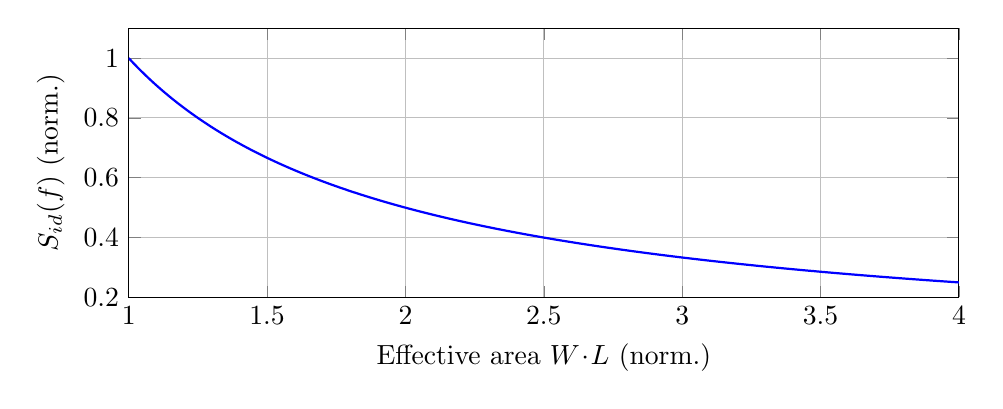
\begin{tikzpicture}
\begin{axis}[
  width=\linewidth,
  height=5cm,
  xlabel={Effective area $W\!\cdot\!L$ (norm.)},
  ylabel={$S_{id}(f)$ (norm.)},
  xmin=1, xmax=4,
  ymin=0.2, ymax=1.1,
  grid=both,
]
\addplot+[thick, mark=none, domain=1:4, samples=200] {1/x};
\end{axis}
\end{tikzpicture}
\caption{Noise versus device area, following $S_{id}\propto 1/(WL)$.}
\label{fig:area}
\end{figure}

% ---------- Figure 4: Long-term stability ----------
\begin{figure}[t]
\centering
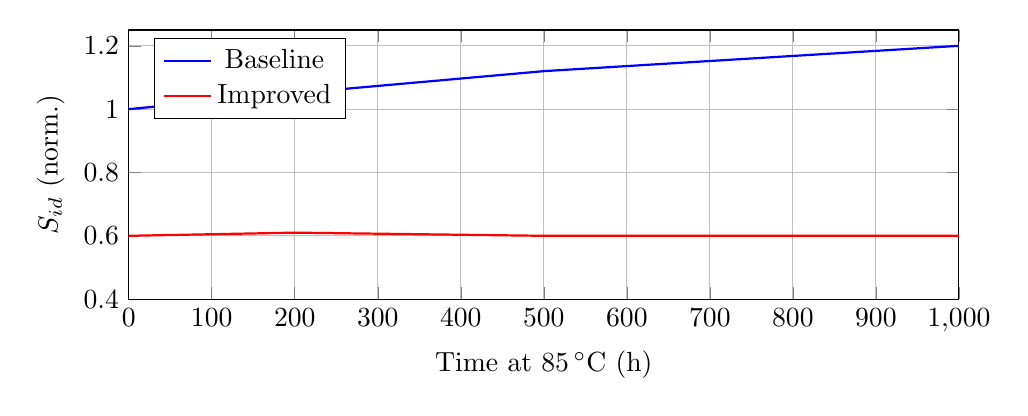
\begin{tikzpicture}
\begin{axis}[
  width=\linewidth,
  height=5cm,
  xlabel={Time at \SI{85}{\celsius} (h)},
  ylabel={$S_{id}$ (norm.)},
  xmin=0, xmax=1000,
  ymin=0.4, ymax=1.25,
  grid=both,
  legend pos=north west
]
\addplot+[thick, mark=none] coordinates {(0,1.0) (200,1.05) (500,1.12) (1000,1.20)};
\addlegendentry{Baseline}
\addplot+[thick, mark=none] coordinates {(0,0.6) (200,0.61) (500,0.60) (1000,0.60)};
\addlegendentry{Improved}
\end{axis}
\end{tikzpicture}
\caption{Long-term stability at \SI{85}{\celsius}: improved split remains stable; baseline drifts $\sim$20\%.}
\label{fig:aging}
\end{figure}

% ---------- 5. Applications ----------
\section{Applications}
Medical EEG/ECG front-ends benefit from improved SNR at low power. MEMS and image sensors gain lower dark/low-frequency noise. Automotive analog (CAN/LIN transceivers, audio, PMIC error amplifiers) demand long-term stability; process-based noise reductions align with AEC-Q100 style reliability.

% ---------- 6. Discussion ----------
\section{Discussion}
Compared with design-only methods, process-based techniques provide fundamental noise reduction without proportional area/power penalties, at the expense of process cost/throughput trade-offs. For mature nodes, such differentiation offers sustainable competitiveness and clear educational value---demonstrating how process/device co-optimization maps to circuit metrics.

% ---------- 7. Conclusion ----------
\section{Conclusion}
A manufacturing strategy combining Epi substrate, oxide/interface engineering, hydrogen anneal, and geometry choices achieves over 50\% reduction in 1/f noise at the \SI{0.18}{\micro\meter} node. The approach is robust across temperature and aging, and its didactic value makes it suitable for curricula and industrial training.

% ---------- References ----------
\section*{References}
\begin{thebibliography}{10}

\bibitem{Sze}
S.~M. Sze and K.~K. Ng, \emph{Physics of Semiconductor Devices}, 3rd~ed. Wiley, 2006.

\bibitem{Razavi}
B.~Razavi, \emph{Design of Analog CMOS Integrated Circuits}. McGraw-Hill, 2001.

\bibitem{Enz}
C.~Enz and G.~C. Temes, ``Circuit techniques for reducing the effects of op-amp imperfections: autozeroing, correlated double sampling, and chopper stabilization,'' \emph{Proc. IEEE}, vol.~84, no.~11, pp. 1584--1614, 1996.

\bibitem{Ziel}
A.~van der Ziel, ``Noise in solid-state devices and lasers,'' \emph{Proc. IEEE}, vol.~58, no.~8, pp. 1178--1206, 1970.

\bibitem{Taur}
Y.~Taur and T.~H. Ning, \emph{Fundamentals of Modern VLSI Devices}, 2nd~ed. Cambridge Univ. Press, 2009.

\bibitem{Takeda}
E.~Takeda and N.~Suzuki, ``Theoretical basis for interface-trap induced MOSFET noise,'' \emph{IEEE Trans. Electron Devices}, vol.~26, no.~5, pp. 784--786, 1979.

\bibitem{Ghibaudo}
G.~Ghibaudo, ``Low frequency noise and fluctuations in advanced CMOS devices,'' \emph{Microelectronics Reliability}, vol.~40, no.~4--5, pp. 587--598, 2000.

\end{thebibliography}

% ---------- Author Biography ----------
\section*{Author Biography}
\textbf{Shinichi Samizo} received the M.S. degree in Electrical and Electronic Engineering from Shinshu University, Japan. He worked at Seiko Epson Corporation on semiconductor memory and mixed-signal device development and contributed to inkjet MEMS actuators and PrecisionCore printhead technology. He is currently an independent semiconductor researcher focusing on process/device education, memory architecture, and AI system integration.\\[2pt]
\emph{Contact:} \href{mailto:shin3t72@gmail.com}{shin3t72@gmail.com}\quad
\emph{GitHub:} \href{https://github.com/Samizo-AITL}{Samizo-AITL}.

\end{document}
